\chapter{Literature Review}\label{ch:literature}

This chapter reviews the work on which the project builds. \Cref{sec:lit-generative} summarises diffusion and flow-matching models and the transformer backbones that are accelerated in this report. \Cref{sec:lit-accel} places training-free caching among the other families of acceleration methods. \Cref{sec:lit-caching,sec:lit-seacache,sec:lit-forecast} review caching in detail, organised by the two decisions every cache makes: \emph{when} to evaluate the network and \emph{what} to write on the steps it skips. SeaCache and Spectrum, the two methods closest to this project, are discussed in depth. \Cref{sec:lit-filtering} covers the estimation theory (Kalman filtering and smoothing) on which KalSea rests, and \cref{sec:lit-mech} surveys diffusion models in mechanical engineering, the target of the applications in \cref{ch:applications}. The chapter closes with the research gaps that motivated ReSPect and KalSea (\cref{sec:lit-gaps}).

%% ------------------------------------------------------------------------------------------------
\section{Diffusion and flow-matching generative models}\label{sec:lit-generative}

\paragraph{Denoising diffusion.} Diffusion models were introduced by \citet{sohl2015deep} as a sequence of small Gaussian perturbations that gradually destroys the structure of the data, together with a learned reverse process that restores it. \citet{ho2020ddpm} made the approach practical with denoising diffusion probabilistic models (DDPM): a network is trained to predict the noise added to a clean sample at a randomly chosen noise level, and sampling runs the learned reverse chain over hundreds to a thousand steps. \citet{song2021sde} unified diffusion and score matching through stochastic differential equations and showed that every diffusion process has a deterministic \emph{probability-flow} ordinary differential equation (ODE) with the same marginals. Deterministic samplers integrate this ODE: DDIM \citep{song2021ddim} reduces the number of steps to tens, and the EDM framework of \citet{karras2022edm} separates the design choices of noise schedule, network preconditioning and solver (with a second-order Heun sampler). Improvements to the noise schedule, such as the cosine schedule of \citet{nichol2021improved} and the zero-terminal-SNR rescaling of \citet{lin2024zerosnr}, are used by several of the models in this report.

\paragraph{Latent diffusion and guidance.} Latent diffusion models \citep{rombach2022ldm} run the diffusion process in the compressed latent space of an autoencoder, which makes high-resolution generation affordable; all image and video models in this report, as well as the topology-optimisation model of \cref{ch:applications}, are latent models. Conditional generation is usually sharpened by classifier-free guidance \citep{ho2022cfg}, which combines a conditional and an unconditional network evaluation at every step and therefore doubles the sampling cost, or is distilled into a single guidance-conditioned evaluation, as in FLUX.1-dev.

\paragraph{Flow matching and rectified flow.} Flow matching \citep{lipman2023flow}, rectified flow \citep{liu2023rectifiedflow} and stochastic interpolants \citep{albergo2023stochastic} learn a velocity field that transports noise to data along (nearly) straight paths $x_\sigma = (1-\sigma)x_\star + \sigma\epsilon$. Sampling integrates the learned velocity with Euler steps over a decreasing schedule of $\sigma$. Scaled to large transformers \citep{esser2024sd3}, this formulation is the basis of the current open text-to-image and text-to-video models.

\paragraph{Diffusion transformers.} Early diffusion models used convolutional U-Nets \citep{ronneberger2015unet,dhariwal2021diffusion}. \citet{peebles2023dit} replaced the U-Net by a transformer \citep{vaswani2017attention} operating on a sequence of latent patches, with the timestep (and class) injected by adaptive layer normalisation (adaLN), and showed that quality improves steadily with model size. The models accelerated in this report are diffusion transformers (DiTs):
\begin{itemize}
  \item \textbf{FLUX.1-dev} \citep{bfl2024flux}, a rectified-flow text-to-image model with 19 double-stream blocks (separate image and text streams with joint attention) followed by 38 single-stream blocks, and guidance distilled into the network;
  \item \textbf{HunyuanVideo} \citep{kong2024hunyuanvideo}, a large text-to-video DiT with a similar dual-/single-stream design;
  \item \textbf{Wan2.1} \citep{wan2025wan}, a text-to-video DiT family (the 1.3B model is used here) sampled with classifier-free guidance and a multistep UniPC solver \citep{zhao2023unipc}.
\end{itemize}
Generating one image or video with these models requires tens of sequential evaluations of a network with billions of parameters over thousands of tokens, which is the cost that this project reduces.

%% ------------------------------------------------------------------------------------------------
\section{Approaches to faster sampling}\label{sec:lit-accel}

The cost of sampling is (number of network evaluations) $\times$ (cost per evaluation). Existing acceleration methods attack one or both factors.

\paragraph{Fast solvers.} Higher-order and multistep ODE solvers reduce the number of steps needed for a given accuracy: DDIM \citep{song2021ddim}, the Heun sampler of EDM \citep{karras2022edm}, DPM-Solver and DPM-Solver++ \citep{lu2022dpmsolver,lu2025dpmsolverpp}, and the predictor--corrector framework UniPC \citep{zhao2023unipc}. Below roughly ten to twenty steps, however, the truncation error of any solver becomes visible.

\paragraph{Distillation.} Progressive distillation \citep{salimans2022progressive}, consistency models \citep{song2023consistency}, latent consistency models \citep{luo2023lcm}, adversarial diffusion distillation \citep{sauer2024add} and distribution matching distillation \citep{yin2024dmd} train a student that samples in one to a few steps. They are very effective but require an expensive training run per model and change the model's outputs.

\paragraph{Quantisation and efficient architectures.} Post-training quantisation such as Q-Diffusion \citep{li2023qdiffusion} and ViDiT-Q \citep{zhao2024viditq} lowers the cost of each evaluation, as do efficient attention kernels.

\paragraph{Feature caching.} Caching exploits the strong similarity of the network's internal activations at consecutive sampling steps: on some steps, all or part of the network is skipped and its output is approximated from steps that were computed. Caching is \emph{training-free}, leaves the weights and the sampler unchanged, and is complementary to the approaches above. Every cache makes two coupled decisions \citep{chung2026seacache}:
\begin{enumerate}
  \item a \textbf{schedule} (or gate) decides \emph{when} the network is evaluated, and
  \item a \textbf{reconstructor} (or filler) decides \emph{what} is written to the features on the steps it skips.
\end{enumerate}
The two are coupled through the length of the skipped runs: a content-aware gate cannot preserve quality on long skips if the skipped features are a stale copy, and an accurate long-horizon predictor cannot be used aggressively if the gate responds to noise rather than to content.

%% ------------------------------------------------------------------------------------------------
\section{Training-free feature caching}\label{sec:lit-caching}

\subsection{Caching in U-Nets and diffusion transformers}
DeepCache \citep{ma2024deepcache} observed that the high-level features of a U-Net change slowly across steps and recomputed only the shallow branch on most steps; block caching \citep{wimbauer2024blockcache} reuses the outputs of individual blocks whose change is predicted to be small. For diffusion transformers, $\Delta$-DiT \citep{chen2024deltadit} caches the deviation of block outputs at the front or back of the network depending on the sampling stage, FORA \citep{selvaraju2024fora} reuses the attention and MLP outputs at a fixed interval, and ToCa \citep{zou2025toca} selects individual tokens to recompute. Video models add a temporal axis of redundancy: Pyramid Attention Broadcast (PAB) \citep{zhao2024pab} broadcasts attention outputs at different rates for spatial, temporal and cross attention, and FasterCache \citep{lv2025fastercache} reuses features and the guidance branch. Learning-to-Cache \citep{ma2024l2c} learns which layers to cache, and OmniCache \citep{chu2025omnicache} distributes reuse globally over the sampling trajectory and filters the noise that reuse introduces.

\subsection{Dynamic gates: deciding when to compute}
Fixed-interval caches spend computation uniformly, although the network output changes quickly at some stages of sampling and slowly at others. Dynamic gates decide online. AdaCache \citep{kahatapitiya2025adacache} adapts the caching schedule to each video using a motion-aware signal. TeaCache \citep{liu2025teacache} accumulates the relative $\ell_1$ change of the timestep-modulated input of the first transformer block, which is available before the expensive blocks run, and recomputes once the sum exceeds a threshold $\delta$; on skipped steps it adds the last computed \emph{residual} of the block stack. MagCache \citep{ma2025magcache} models the magnitude ratio of successive residuals, DiCache \citep{bu2025dicache} probes a shallow layer to estimate the change of the deep features, and FreqCa \citep{liu2025freqca} treats frequency bands differently. These gates use the raw change of a feature as the signal. As argued in the ReSPect paper, this raw distance is a noise-contaminated drift: at early steps the noise contribution can dominate it, so the gate reacts to stochastic variation rather than to the evolving content.

%% ------------------------------------------------------------------------------------------------
\section{SeaCache: a spectrally aligned gate}\label{sec:lit-seacache}

SeaCache \citep{chung2026seacache} keeps TeaCache's accumulate-and-reset rule but measures the change \emph{after} a spectral-evolution-aware (SEA) filter. Modelling the latent at step $t$ as $x_t = a_t x_0 + b_t\epsilon$ with white noise $\epsilon$, the linear minimum-mean-square-error estimator of $x_0$ from $x_t$ is a convolution whose frequency response is the Wiener filter
\begin{equation}
  G_t(f) = \frac{a_t S_x(f)}{a_t^2 S_x(f) + b_t^2},
\end{equation}
where $S_x$ is the power spectrum of clean latents. Under a power-law prior $S_x(f)\propto |f|^{-\beta}$, $G_t$ is a low-pass filter at early (noisy) steps and admits progressively higher frequencies as sampling proceeds, reproducing the well-known coarse-to-fine evolution of diffusion sampling. SeaCache filters the first block's modulated input with the gain-normalised $G_t$ for the current noise level and accumulates the relative $\ell_1$ change of the filtered input, so that the gate responds to content rather than noise. It uses $\beta=2$ for images and $\beta=3$ for videos, always computes the first and last steps, and on skipped steps \emph{reuses} the last computed residual. The full derivation is given in \cref{sec:bg-sea}.

During this project two observations about SeaCache became important. First, its reconstructor is plain reuse, whose error grows linearly with the skip length (\cref{ch:respect}); SeaCache improves \emph{when} to compute but not \emph{what} to write. Second, its released HunyuanVideo script binds the scheduler that exists when the model is loaded, whereas the HunyuanVideo sampler creates a fresh scheduler for sampling. The gate therefore reads a stale noise level close to one instead of the sampling schedule, which skips step 1 once $\delta\gtrsim 0.21$ and costs 12--14\,dB on the affected prompts. KalSea reads the live noise level of the sampler (\cref{ch:kalsea}).

%% ------------------------------------------------------------------------------------------------
\section{Forecasting and correcting skipped features}\label{sec:lit-forecast}

\subsection{From reuse to forecasting}
Reuse is a zero-order prediction. TaylorSeer \citep{liu2025taylorseer} replaces it by a Taylor extrapolation built from finite differences of the features cached at the most recent computed steps, which is accurate for short skips but uses only local information and amplifies noise at higher orders. HiCache \citep{feng2026hicache} replaces the Taylor basis by scaled Hermite polynomials. FoCa \citep{zheng2026foca} treats feature caching as an ODE and combines a second-order backward-differentiation predictor with a Heun-type calibration.

\subsection{Spectrum: global Chebyshev forecasting}
Spectrum \citep{han2026spectrum} forecasts the hidden-state trajectory globally. The solver index is mapped affinely to $\tau\in[-1,1]$, every feature channel is expanded in Chebyshev polynomials $T_0,\dots,T_M$ (\cref{fig:lit-chebyshev}), and the coefficients are fitted by ridge regression \citep{hoerl1970ridge} to all features recorded so far. The forecast at a skipped step evaluates the fitted expansion at its coordinate, and is blended with a first-order discrete Taylor step. Spectrum's analysis gives three results that ReSPect builds on: an order-$(P{+}1)$ remainder for an ideal degree-$P$ Taylor predictor, a truncation error of the Chebyshev expansion that decays as $\rho^{-M}$ for functions analytic in a Bernstein ellipse and is independent of the skip length \citep{trefethen2019approximation}, and a stability bound for the ridge estimator. Spectrum forecasts the full hidden state and is used with simple schedules.

\begin{figure}[t]
  \centering
  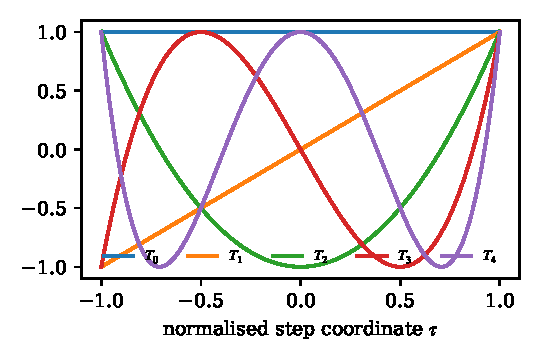
\includegraphics[width=0.55\textwidth]{lit_chebyshev.pdf}
  \caption[Chebyshev polynomials used by Spectrum and ReSPect]{The Chebyshev polynomials $T_0,\dots,T_4$ on the normalised step coordinate $\tau\in[-1,1]$. Spectrum and ReSPect fit each feature channel with a ridge-regularised expansion in this basis ($M=4$).}
  \label{fig:lit-chebyshev}
\end{figure}

\subsection{Correcting what is written}
Several recent methods check or repair the values written on skipped steps. SpeCa \citep{liu2025speca} accepts or rejects each forecast with a lightweight verification, OmniCache \citep{chu2025omnicache} filters the noise introduced by reused features, ERTACache \citep{peng2026ertacache} adjusts the integration intervals and rectifies cache-induced errors with a closed-form model profiled offline, and GP-Refiner \citep{shen2026gprefiner} regresses the deviation of forecast features online with a Gaussian process. Contemporaneous with KalSea, SpecKCast \citep{rajabi2026speckcast} tracks the DCT coefficients of the \emph{model output} with damped-trend Kalman filters along band-specific warped time and schedules computation by the filter's uncertainty. All of these methods improve the value used at the current or upcoming steps; none of them revises the latent of steps that have already been skipped. This observation is the starting point of KalSea (\cref{ch:kalsea}).

%% ------------------------------------------------------------------------------------------------
\section{Filtering, smoothing and predictor--corrector integration}\label{sec:lit-filtering}

The Kalman filter \citep{kalman1960} is the exact recursive minimum-mean-square-error estimator of the state of a linear-Gaussian state-space model; the Rauch--Tung--Striebel (RTS) smoother \citep{rauch1965rts} computes the estimates of past states given all observations, including later ones. Both are covered in the textbook of \citet{sarkka2013bayesian}. In target tracking, the integrated Wiener process (constant-velocity) model with state (position, velocity) is standard \citep{barshalom2001estimation}; damping the velocity, as in the damped-trend models of exponential smoothing \citep{gardner1985damped}, prevents forecasts over long horizons from overshooting, and the process-noise intensity can be adapted online so that the observed innovations match their predicted variance \citep{mehra1972adaptive}. Probabilistic ODE solvers \citep{schober2019probabilistic,tronarp2019probabilistic} infer the solution of an ODE from evaluations of its vector field by Gauss--Markov filtering and smoothing. In diffusion sampling, predictor--corrector schemes add Langevin steps \citep{song2021sde} or a second evaluation \citep{karras2022edm}, and UniPC \citep{zhao2023unipc} corrects a multistep solver by reusing the next network evaluation, which the sampler performs anyway. KalSea uses the RTS smoother for a different purpose: to infer the network evaluations that a cache \emph{skipped}.

%% ------------------------------------------------------------------------------------------------
\section{Diffusion models in mechanical engineering}\label{sec:lit-mech}

Deep generative models have become a design tool in mechanical engineering \citep{regenwetter2022deep}. Two application areas are relevant to this report.

\paragraph{Structural topology optimisation.} Topology optimisation distributes material in a design domain so as to minimise compliance (maximise stiffness) under loads, supports and a volume constraint. The homogenisation method of \citet{bendsoe1988generating} and density-based SIMP implementations such as the 99-line and 88-line codes \citep{sigmund2001,andreassen2011efficient} require a finite-element analysis at each of many iterations, which makes the optimisation expensive for large or repeated problems. Generative models learn to propose near-optimal structures directly. TopoDiff \citep{maze2023topodiff} showed that a conditional diffusion model guided by physical fields and surrogate models produces better structures than GAN-based approaches. \citet{giannone2023aligning} align the sampling trajectory of the diffusion model with the trajectory of the optimiser, and NITO \citep{nobari2024nito} uses neural implicit fields for resolution-free topology optimisation. Optimize Any Topology (OAT) \citep{nobari2025oat} combines a resolution- and shape-agnostic neural-field autoencoder with a conditional latent diffusion model trained on OpenTO, a dataset of 2.2 million optimised structures, and predicts minimum-compliance layouts for arbitrary aspect ratios, resolutions, volume fractions, loads and fixtures. Its denoiser is a conditional U-Net sampled with DDIM, and its code and weights are public, which makes it the first application in \cref{ch:applications}. Diffusion models are also used for other design tasks, such as boundary-representation CAD models \citep{xu2024brepgen} and mechanical metamaterials with a prescribed nonlinear response \citep{bastek2023inverse}.

\paragraph{Fluid mechanics and PDE-governed fields.} Physics-informed neural networks \citep{raissi2019pinn} and neural operators such as the Fourier neural operator \citep{li2021fno} learn solutions of partial differential equations (PDEs). Diffusion models add the ability to represent uncertainty and to reconstruct fields from incomplete data: \citet{shu2023physics} reconstruct high-fidelity flow fields from low-fidelity inputs with a physics-informed diffusion model, and \citet{kohl2023benchmarking} benchmark autoregressive conditional diffusion models for turbulent flow simulation. DiffusionPDE \citep{huang2024diffusionpde} learns the joint distribution of PDE coefficients (or initial states) and solutions with an EDM model and solves forward and inverse problems from sparse observations by guiding the sampler with the observation loss and the PDE residual, in the manner of diffusion posterior sampling \citep{chung2023dps}. Its sampler uses 2000 guided second-order steps, so sampling is the dominant cost, which makes it the second application in \cref{ch:applications}.

In both areas the generative model is evaluated many times per design or per solution, and design studies require many designs. Acceleration that is training-free and leaves the model unchanged is therefore directly useful, yet caching methods have so far been developed and evaluated almost exclusively on text-to-image and text-to-video models.

%% ------------------------------------------------------------------------------------------------
\section{Research gaps}\label{sec:lit-gaps}

\Cref{tab:lit-summary} summarises the caching methods along the two decisions of a cache. The review identifies the following gaps.
\begin{enumerate}
  \item \textbf{Gate and reconstructor are improved in isolation.} SeaCache improves the gate but keeps reuse; Spectrum improves the reconstructor but uses simple schedules. Since the two decisions are coupled through the skip length, neither can realise its benefit alone.
  \item \textbf{The regression target is larger than necessary.} Forecasting methods predict the full hidden state, although on a skipped step the block input is known exactly and only the block-stack residual is missing.
  \item \textbf{Hyper-parameters of forecasters are tuned empirically,} for example the blend between a local and a global predictor and the number of warm-up steps.
  \item \textbf{All fillers are open loop.} Reuse and every forecaster predict the skipped steps from the past only. When the next computed step reveals the error, the sampler has already integrated it into the latent, and no existing method revises the latent of the skipped steps.
  \item \textbf{Engineering diffusion models have not been accelerated by caching,} even though they are sampled with many steps and used in loops over many designs.
\end{enumerate}
ReSPect (\cref{ch:respect}) addresses gaps 1--3: it couples the SEA gate with a residual forecaster whose blend and warm-up are derived analytically. KalSea (\cref{ch:kalsea}) addresses gap 4 with predictor--corrector gap smoothing, and \cref{ch:applications} addresses gap 5.

\begin{table}[t]
  \centering
  \small
  \caption[Summary of training-free caching methods]{Training-free caching methods by their two decisions. ``Loop'': whether the error of the filler on skipped steps is corrected once the next computed step is observed.}
  \label{tab:lit-summary}
  \begin{tabularx}{\textwidth}{@{}l>{\raggedright\arraybackslash}X>{\raggedright\arraybackslash}Xl@{}}
    \toprule
    Method & When to compute (schedule) & What to write (filler) & Loop \\
    \midrule
    DeepCache, block caching & fixed / block-wise & reuse of U-Net features & open \\
    $\Delta$-DiT, FORA, ToCa, PAB & fixed interval, block / token level & reuse & open \\
    TeaCache, MagCache, DiCache & accumulated raw change & reuse of residual & open \\
    SeaCache & accumulated SEA-filtered change & reuse of residual & open \\
    TaylorSeer, HiCache & fixed interval & Taylor / Hermite extrapolation & open \\
    Spectrum & fixed / simple & Chebyshev ridge + Taylor (hidden state) & open \\
    FoCa & fixed interval & BDF2 predictor + Heun calibration & open \\
    SpecKCast & filter uncertainty & Kalman forecast of DCT output & open \\
    \midrule
    \textbf{ReSPect} (ours) & accumulated SEA-filtered change & Chebyshev ridge + Taylor (\emph{residual}), analytic blend & open \\
    \textbf{KalSea} (ours) & accumulated SEA-filtered change & Kalman forecast of residual + \emph{PCGS} & \textbf{closed} \\
    \bottomrule
  \end{tabularx}
\end{table}
